%%==================================================================%%
%% Author : Sa�udo Olmedo, Ignacio                                  %%
%% Author : S�nchez Barreiro, Pablo                                 %%
%% Version: 1.2, 15/05/2014                                         %%
%%                                                                  %%
%% Memoria del Proyecto Fin de Carrera                              %%
%% Cap�tulo m2t, Archivo ra�z                                       %%
%%==================================================================%%

\chapterheader{Transformaci�n modelo a texto}{Transformaci�n modelo a texto}
\label{chap:m2t}

El cap�tulo anterior describi� el funcionamiento y desarrollo del primer paso del proceso de transformaci�n dirigido por modelos, 'Model To model' (M2M). En este cap�tulo se presenta el siguiente paso del proceso de transformaci�n dirigido por modelos, dicho paso consiste en la transformaci�n del modelo a texto, este paso es mas conocido como 'Model To Text' (M2T). En este capitulo se explica como se ha realizado la implementaci�n del generador de c�digo utilizando para ello el lenguaje Epsilon Generation Language (EGL). Este cap�tulo describe el funcionamiento y desarrollo de los generadores de c�digo, los cuales tienen como objetivo adaptar la implementaci�n de referencia a las necesidades de cada cliente.

\chaptertoc

\section{Introducci�n}
\label{m2t:sec:intro}
%%==================================================================%%
%% Author : Sa�udo Olmedo, Ignacio                                  %%
%%          S�nchez Barreiro, Pablo                                 %%
%% Version: 1.3, 18/06/2014                                         %%
%%                                                                  %%
%% Memoria del Proyecto Fin de Carrera                              %%
%% Antecedentes/Introducci�n                                        %%
%%==================================================================%%





\section{Generador de c�digo}
\label{m2t:sec:intro}
%%==================================================================%%
%% Author : Sa�udo Olmedo, Ignacio                                  %%
%% Author : S�nchez Barreiro, Pablo                                 %%
%% Version: 1.5, 15/05/2014                                         %%
%%                                                                  %%
%% Memoria del Proyecto Fin de Carrera                              %%
%% m2t/Sumario                                                      %%
%%==================================================================%%

Esta secci�n analiza el proceso de creaci�n del generador de c�digo. El desarrollo del generador de c�digo se ha realizado con el lenguaje Epsilon Generation Language (EGL), este lenguaje es utilizado para la generaci�n de c�digo basado en la transformaci�n de modelos, el lenguaje a generar es Cassandra Query Language (CQL). Este lenguaje de consultas es muy similar a SQL, sin embargo existen peque�as diferencias que se han citado a lo largo del proyecto por ejemplo: la definici�n de claves, tipos de dato etc.

El proceso de transformaci�n modelo-c�digo es el siguiente.
En primer lugar se realiza la definici�n del keyspace para ello hay que tomar el nombre del keyspace que parte del modelo transformado Cassandra y la estrategia de replicaci�n (ver capitulo 3, secci�n 2).
A continuaci�n se define la creaci�n de una column family en CQL. Tras determinar el bloque de creaci�n de la column family (CREATE TABLE) se definen las columnas de la tabla. Por cada columna de la column family se obtiene el nombre de la columna y se fija el tipo de dato de la columna (primitivo,map,set/list) junto con su nombre. La definici�n de estas columnas ser�a la siguiente.
\begin{enumerate}
\item Tipo b�sico: "nombre columna-tipo primitivo".
\item Map: "nombre columna-map-(tipo primitivo 1,tipo primitivo 2)".
\item Set/list: "nombre columna-set-tipo primitivo)".
\end{enumerate}
En la figura~\ref{back:code:m2t} se muestra parte del c�digo para realizar esto (lenguaje ETL). El resto de c�digo se ha omitido por razones de espacio sin embargo se detalla a continuaci�n.

Tras la definici�n de la columna se define la primary key. Para la definici�n de la primary key debemos diferenciar si la column family es din�mica o est�tica. En caso de ser est�tica la definici�n ser�a la cl�sica: PRIMARY KEY(ColumnaClave).
En el caso de tratarse de una column family din�mica la construcci�n modelo-c�digo es distinta, la m�s frecuente es la siguiente: PRIMARY KEY(partitioning key, clustering key\_1 ... clustering key\_n)
Sin embargo hay que tener en cuenta que en la construcci�n y seg�n la documentaci�n de CQL tambi�n es posible tener una partition key compuesta, es decir, una partition key formada por varias columnas, para realizar esto se utilizan par�ntesis y as� delimitamos el conjunto de partici�n. Quedando una posible definici�n de la primary key de la siguiente manera: PRIMARY KEY((partitioning key\_1, ... partitioning key\_n), clustering key\_1 ... clustering key\_n). Este proceso se repite por cada column family del modelo.

\begin{figure}[!tb]
\begin{center}
\begin{footnotesize}
\begin{verbatim}
--------------------------------------------------------
DROP KEYSPACE [%=keyspace.name%];
CREATE KEYSPACE [%=keyspace.name%]
WITH replication = {'class':'[%=keyspace.replicaPlacementStrategy%]', 'replication_factor':[%=keyspace.replicationFactor%]};

USE [%=keyspace.name%];

[% for (cf in keyspace.columnFamilies){ tableKey="";%]
CREATE TABLE [%=cf.name%](
	[% for (cols in cf.columns){ //este for define cada grupo de columnas
		s=cols.name.toString();
		for (c in cols.type){
		
			if (c.isTypeOf(PrimitiveType))  //definicion del tipo primitivo
				s=s+" "+c.kind.toString();
				
			if (c.isTypeOf(MapType)) //definicion del tipo map
				s=s+" Map"+"<"+c.keyType.toString()+","+c.baseType.toString()+">";
				
 			if(c.isTypeOf(CollectionType)) //definicion del tipo set o list
				s=s+" "+c.kind.toString()+"<"+c.keyType.toString()+">";
			
		}
);
[%}%]
--------------------------------------------------------
\end{verbatim}
\end{footnotesize}
\end{center}
\caption{Regla de transformaci�n Primary Key}
\label{back:code:m2t}
\end{figure}

Una vez definido el c�digo EGL podemos poner en funcionamiento el generador de c�digo. El proceso completo ser�a el siguiente: En primer lugar creamos un modelo UML con cualquier herramienta de modelado, por ejemplo el modelo UML de Twissandra ha sido realizado con la herramienta Magic Draw. A continuaci�n transformamos este modelo UML al modelo Cassandra con los m�todos de transformaci�n definidos en el cap�tulo anterior, una vez obtenido este modelo de Cassandra podemos poner en funcionamiento el generador de c�digo, este proceso con el caso de estudio de Twissandra es descrito en la siguiente secci�n. Con el c�digo ya generado podemos crear el repositorio de datos Cassandra. 

\section{Caso de estudio Twissandra}
\label{m2t:sec:tw}
%%==================================================================%%
%% Author : Sa�udo Olmedo, Ignacio                                  %%
%% Author : S�nchez Barreiro, Pablo                                 %%
%% Version: 1.5, 15/05/2014                                         %%
%%                                                                  %%
%% Memoria del Proyecto Fin de Carrera                              %%
%% m2t/Caso de estudio                                              %%
%%==================================================================%%

Una vez definido el funcionamiento del generador de c�digo podemos continuar con el caso de estudio planteado en el segundo cap�tulo sobre Twissandra. Como se present� anteriormente el objetivo de este caso de estudio es la generaci�n de c�digo CQL a partir de un modelo UML 2.0. Para ello definimos una serie de reglas de transformaci�n entre modelos y obtuvimos un modelo de Cassandra a partir de un modelo UML que representaba una versi�n simplificada de Twitter llamada Twissandra.
En esta secci�n se presenta el resultado de la transformaci�n del modelo de Twissandra a c�digo.

Tras obtener el modelo Cassandra de Twissandra (figura~\ref{back:fig:modeloTwissandra}) y tras la definici�n del generador de c�digo se pone en funcionamiento la transformaci�n modelo-c�digo. El resultado de la transformaci�n se detalla a continuaci�n.El c�digo resultante tras ejecutar el generador de c�digo es el siguiente (figura~\ref{back:code:codigoCass}).

\begin{figure}[!tb]
  \centering
  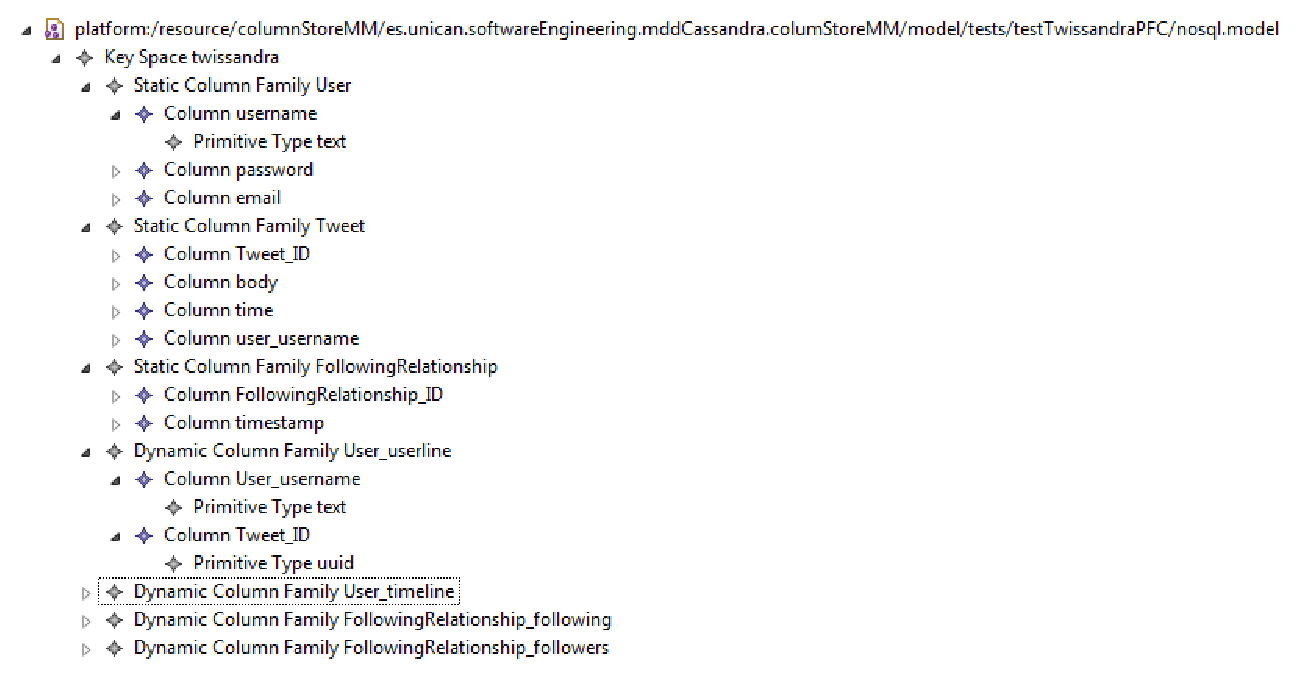
\includegraphics[width=.8\linewidth]{m2t/images/modeloTwissandra.eps} \\
  \caption{Modelo UML Twissandra}
  \label{back:fig:modeloTwissandra}
\end{figure}

Como vemos en el c�digo las tres primeras l�neas son para borrar el keyspace en caso de que existiera, crearlo y configurar la arquitectura de replicaci�n seg�n estaba especificado en el modelo Cassandra. A continuaci�n se conecta la sesi�n con el keyspace correspondiente.
Por cada column family (sea est�tica o din�mica) se genera un bloque \"CREATE TABLE\". Cada columna de la column family es transformada en una columna de la tabla. La transformaci�n como se contaba en la secci�n anterior es trivial, sin embargo el problema del generador de c�digo surge a la hora de definir la estructura de la primary key. Las column family est�ticas siguen una definici�n de claves tradicional, sin embargo las column families din�micas tienen que tener en cuenta que las claves de partici�n (partition keys) pueden ser compuestas (aunque en este ejemplo no existen). Por ejemplo el caso de user\_userline las columnas user\_name y tweet\_id son designadas como primary key, user\_username ser� la clave de partici�n.


\begin{figure}[!tb]
\begin{center}
\begin{footnotesize}
\begin{verbatim}
DROP KEYSPACE twissandra;
CREATE KEYSPACE twissandra
WITH replication = {'class':'SimpleStrategy', 'replication_factor':1};

USE twissandra;

CREATE TABLE User(
       username text,
       password text,
       email set<text>,
       PRIMARY KEY(username)
);

CREATE TABLE Tweet(
       Tweet_ID uuid,
       body text,
       time timestamp,
       user_username text,
       PRIMARY KEY(Tweet_ID)
);

CREATE TABLE FollowingRelationship(
       FollowingRelationship_ID uuid,
       timestamp timestamp,
       PRIMARY KEY(FollowingRelationship_ID)
);

CREATE TABLE User_userline(
       User_username text,
       Tweet_ID uuid,
       PRIMARY KEY((User_username),Tweet_ID)
);

CREATE TABLE User_timeline(
       User_username text,
       Tweet_ID uuid,
       PRIMARY KEY((User_username),Tweet_ID)
);

CREATE TABLE FollowingRelationship_following(
       FollowingRelationship_FollowingRelationship_ID uuid,
       username text,
       PRIMARY KEY((FollowingRelationship_FollowingRelationship_ID),username)
);

CREATE TABLE FollowingRelationship_followers(
       FollowingRelationship_FollowingRelationship_ID uuid,
       username text,
       PRIMARY KEY((FollowingRelationship_FollowingRelationship_ID),username)
);

\end{verbatim}
\end{footnotesize}
\end{center}
\caption{C�digo resultante Twissandra}
\label{back:code:codigoCass}
\end{figure}



\section{Pruebas}
\label{m2t:sec:pr}
%%=======================================================================%%
%% Author : Sa�udo Olmedo, Ignacio                                       %%
%% Author : S�nchez Barreiro, Pablo                                      %%                                                                      %%                                                                       %%
%% Version: 2.0, 25/06/2014                                              %%                                                                         %%                                                                       %%
%% Memoria del Proyecto Fin de Carrera                                   %%
%% M2M/Pruebas con EUnit                                                 %%   %%=======================================================================%%

Una vez implementado el generador de c�digo la siguiente tarea consiste en comprobar que el c�digo generado funciona correctamente.
Para ello creamos, una serie de pruebas unitarias que permitan comprobar que el funcionamiento de los generadores de c�digo es correcto para un conjunto de modelos de entrada.

Estas pruebas unitarias se han implementado en EUnit, el lenguaje de definici�n de pruebas de la suite Epsilon. EUnit funciona de una manera muy similar a JUnit, pero aplicado a los lenguajes de la suite Epsilon, como EGL. Utilizamos EUnit para comprobar que el funcionamiento del generador de c�digo es correcto, para ello se dise�an una serie de casos de prueba y se crea la salida esperada de cada uno de esos casos de prueba de forma manual.
A continuaci�n, se ejecuta el caso de prueba creado en EUnit y se comprueba que la salida generada coincide con la esperada, que es la creada manualmente. Adem�s comprobamos con casos espec�ficos que la cobertura del c�digo es del 100%.

El �nico problema surge por un problema de defecto en la herramienta EUnit, la funci�n de comparaci�n de ficheros llamada assertEqualFiles obliga a que ambos ficheros sean estrictamente iguales por lo que para crear casos de prueba tanto el c�digo de entrada de prueba como el c�digo generado a testear han de ser iguales, espacios y saltos de l�nea incluidos.


%\section{Despliegue}
%\label{m2t:sec:des}
%\input{m2t/despliegue.tex}

\section{Sumario}
\label{m2t:sec:sumario}
%%==================================================================%%
%% Author : Sa�udo Olmedo, Ignacio                                  %%
%% Author : S�nchez Barreiro, Pablo                                 %%
%% Version: 1.5, 15/05/2014                                         %%
%%                                                                  %%
%% Memoria del Proyecto Fin de Carrera                              %%
%% m2t/Sumario                                                      %%
%%==================================================================%%

Durante este cap�tulo se ha descrito el proceso de desarrollo del generador de c�digo. En primer lugar se ha presentado el c�digo del generador de c�digo y parte de la sintaxis utilizada para construirlo as� como la descripci�n de su realizaci�n. A continuaci�n se ha descrito el proceso de transformaci�n del caso de estudio introducido en el cap�tulo dos. Finalmente se han presentado las pruebas realizadas as� comola herramienta utilizada.   


